\documentclass[crop, tikz]{standalone}

\usepackage{tikz}
\usepackage{amsmath}
\usepackage{amssymb}
\usepackage[mode=buildnew]{standalone}

\usepackage{xcolor}


\usetikzlibrary{positioning}
\usetikzlibrary{calc}
\usetikzlibrary{fit}
%\usepackage{nicematrix}

\tikzset{set/.style={draw,circle,inner sep=0pt,align=center}}

\definecolor{morange}{RGB}{255,127,14}
\definecolor{mblue}{RGB}{31,119,180}
\definecolor{mred}{RGB}{214,39,40}
\definecolor{mpurple}{RGB}{148,103,189}
\definecolor{mgreen}{RGB}{44,160,44}

\begin{document}
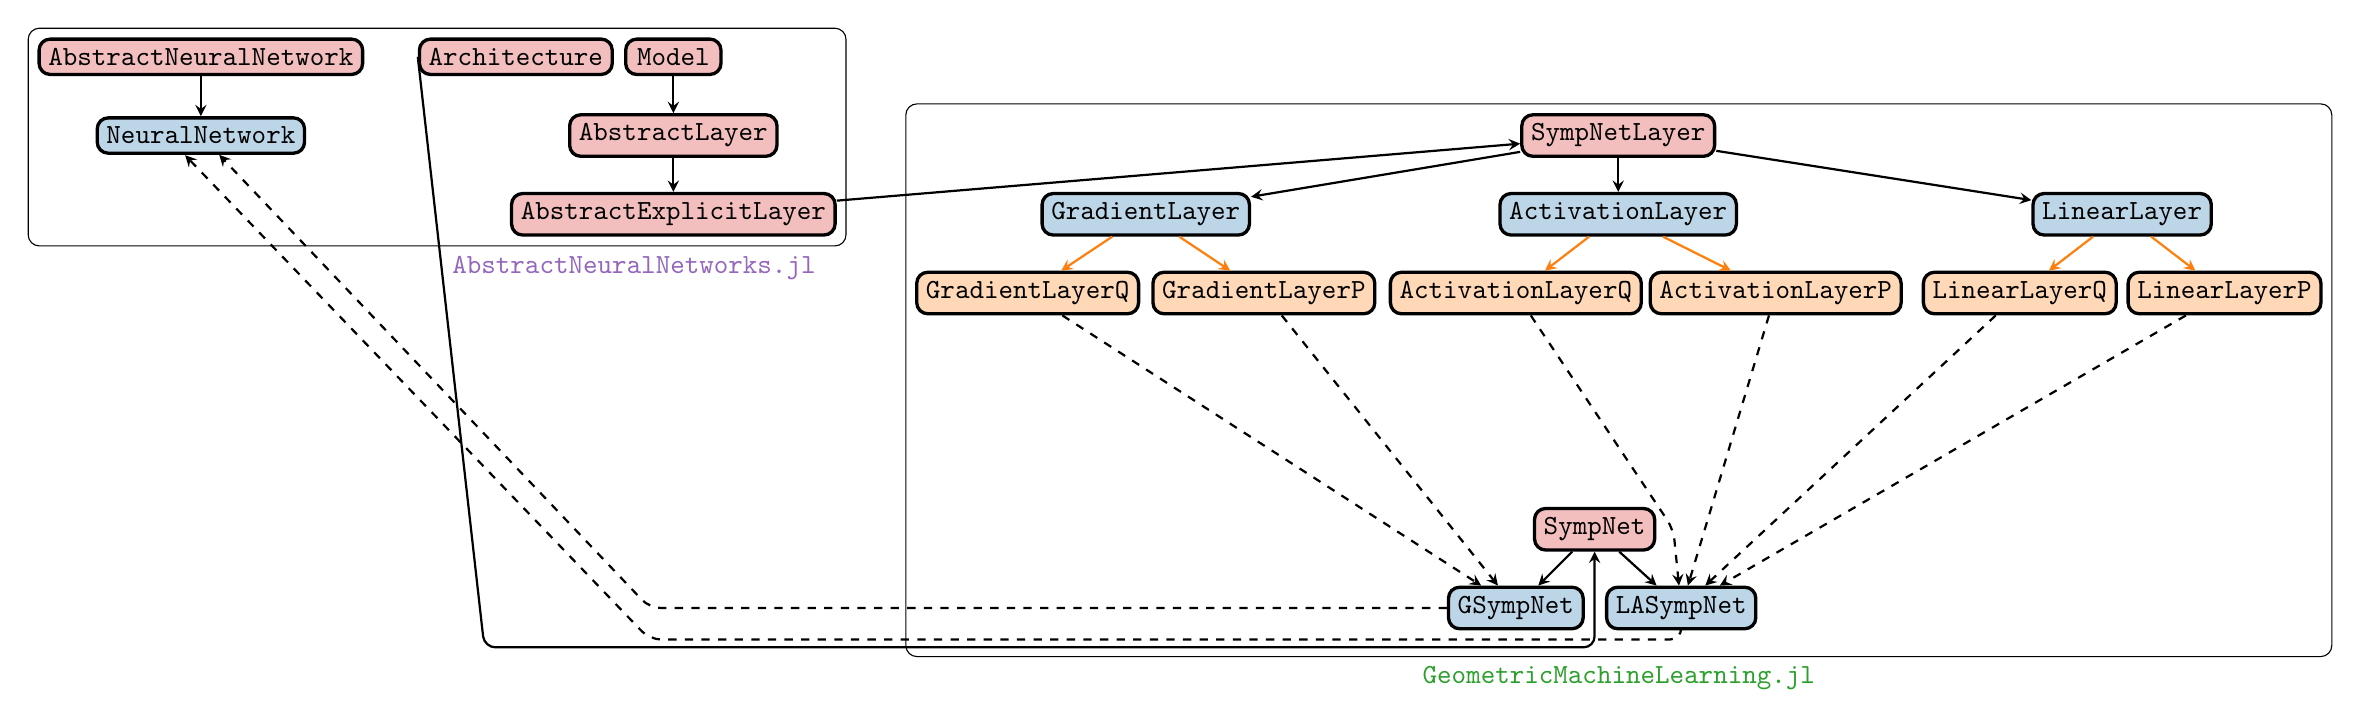
\begin{tikzpicture}[module/.style={draw, very thick, rounded corners, minimum width=8ex},
    abstract_type/.style={module, fill=mred!30},
    chain/.style={module, fill=mgreen!30},
    constructor/.style={module, fill=morange!30},
    struct/.style={module, fill=mblue!30},
    arrow_exp/.style={-stealth, thick, rounded corners},
    arrow_imp/.style={-stealth, thick, rounded corners, dashed},
    arrow_constructor/.style={arrow_exp, morange},
]
%\node[module] (ann) {\texttt{AbstractNeuralNetworks.jl}};
%\node[module, right of=ann, xshift=5cm] (gml) {\texttt{GeometricMachineLearning.jl}};

\node[abstract_type] (architecture) {\texttt{Architecture}};

\node[abstract_type, right of=architecture, xshift=1cm] (model) {\texttt{Model}};
\node[abstract_type, below of=model] (al) {\texttt{AbstractLayer}};
\node[abstract_type, below of=al] (ael) {\texttt{AbstractExplicitLayer}};

\node[abstract_type, left of=architecture, xshift=-3cm] (ann) {\texttt{AbstractNeuralNetwork}};
\node[struct, below of=ann] (nn) {\texttt{NeuralNetwork}};

\node[abstract_type, below of=ael, xshift=12cm, yshift=2cm] (sympnetlayer) {\texttt{SympNetLayer}};
\node[struct, below of=sympnetlayer, xshift=-6cm] (gradient) {\texttt{GradientLayer}};
\node[struct, below of=sympnetlayer] (activation) {\texttt{ActivationLayer}}; 
\node[struct, below of=sympnetlayer, xshift=6.4cm] (linear) {\texttt{LinearLayer}};

\node[constructor, below of=gradient, xshift=-1.5cm] (gradientq) {\texttt{GradientLayerQ}}; 
\node[constructor, below of=gradient, xshift=1.5cm] (gradientp) {\texttt{GradientLayerP}}; 
\node[constructor, below of=activation, xshift=-1.3cm] (activationq) {\texttt{ActivationLayerQ}};
\node[constructor, below of=activation, xshift=2.0cm] (activationp) {\texttt{ActivationLayerP}};
\node[constructor, below of=linear, xshift=-1.3cm] (linearq) {\texttt{LinearLayerQ}};
\node[constructor, below of=linear, xshift=1.3cm] (linearp) {\texttt{LinearLayerP}};

\node[abstract_type, below of=activationq, xshift=1cm, yshift=-2cm] (sympnetnetwork) {\texttt{SympNet}};
\node[struct, below of=sympnetnetwork, xshift=-1cm] (gsympnet) {\texttt{GSympNet}};
\node[struct, below of=sympnetnetwork, xshift=1.1cm] (lasympnet) {\texttt{LASympNet}};

\draw[arrow_exp] (model) -- (al);
\draw[arrow_exp] (al) -- (ael); 

\draw[arrow_exp] (ael) -- (sympnetlayer);
\draw[arrow_exp] (sympnetlayer) -- (gradient);
\draw[arrow_exp] (sympnetlayer) -- (activation); 
\draw[arrow_exp] (sympnetlayer) -- (linear); 

% arrows for the constructor
\draw[arrow_constructor] (gradient) -- (gradientq);
\draw[arrow_constructor] (gradient) -- (gradientp); 
\draw[arrow_constructor] (activation) -- (activationq); 
\draw[arrow_constructor] (activation) -- (activationp);
\draw[arrow_constructor] (linear) -- (linearq);
\draw[arrow_constructor] (linear) -- (linearp);

\coordinate[right of=linearp, yshift=-.3cm] (right_of_linearp);
\coordinate[below of=sympnetnetwork, yshift=-.5cm] (below_of_sympnet);
\coordinate[left of=ael, xshift=-1.4cm, yshift=-5.5cm] (left_of_ael);

\draw[arrow_exp] (architecture.west)--(left_of_ael)--(below_of_sympnet)--(sympnetnetwork);
\draw[arrow_exp] (sympnetnetwork) -- (gsympnet);
\draw[arrow_exp] (sympnetnetwork) -- (lasympnet); 

\coordinate[right of=sympnetnetwork] (right_of_sympnet);

\draw[arrow_imp] (linearq) -- (lasympnet);
\draw[arrow_imp] (linearp) -- (lasympnet);
\draw[arrow_imp] (activationq)--(right_of_sympnet)--(lasympnet);
\draw[arrow_imp] (activationp) -- (lasympnet);
\draw[arrow_imp] (gradientq) -- (gsympnet);
\draw[arrow_imp] (gradientp) -- (gsympnet);

\draw[arrow_exp] (ann) -- (nn);

\coordinate[left of=gsympnet, xshift=-10cm] (left_of_gsympnet);

\draw[arrow_imp] (gsympnet.west)--(left_of_gsympnet)--(nn);

\coordinate[below of=lasympnet, yshift=.6cm] (below_of_lasympnet);
\coordinate[below of=left_of_gsympnet, yshift=.6cm] (left_of_gsympnet2);
\coordinate[left of=nn, xshift=.8cm, yshift=-.25cm] (nn2);

\draw[arrow_imp] (lasympnet.south)--(below_of_lasympnet)--(left_of_gsympnet2)--(nn2);

\node[fit=(architecture)(model)(al)(ael)(ann), label=below:\color{mpurple}\hspace{5cm}\texttt{AbstractNeuralNetworks.jl}, draw, rounded corners] (ann) {};
\node[fit=(sympnetnetwork)(gradient)(gradientq)(gsympnet)(lasympnet)(linearp)(linear)(sympnetlayer)(below_of_sympnet), label=below:\color{mgreen}\texttt{GeometricMachineLearning.jl}, draw, rounded corners] (gml) {}; 


\end{tikzpicture}
\end{document}